% !TeX root = class2-forcefields.tex
\documentclass[11pt]{article}
\usepackage[margin=2.4cm]{geometry}
\usepackage{amsmath}
\usepackage{xcolor}
\usepackage{booktabs}
\usepackage{graphicx}
\usepackage[T1]{fontenc}
\usepackage{lmodern}
\usepackage[numbers]{natbib}
\usepackage{hyperref}
% Colours: one per term, generated by ff_style.py (do not edit chapter/colors.tex by hand).
% Colour appears only in displayed equations, tables and figures.
\definecolor{ffInk}{HTML}{212745}
\definecolor{cBond}{HTML}{1F5FBF}  % bond: class I (anharmonic in class II)
\definecolor{cAngle}{HTML}{00899B}  % angle: class I (anharmonic in class II)
\definecolor{cTorsion}{HTML}{3949AB}  % torsion: class I
\definecolor{cBondBond}{HTML}{E4572E}  % bond-bond: class II cross term
\definecolor{cBondAngle}{HTML}{E0A100}  % bond-angle: class II cross term
\definecolor{cAngleAngle}{HTML}{C2185B}  % angle-angle: class II cross term
\definecolor{cBondTorsion}{HTML}{8C5A2B}  % bond-torsion: class II cross term
\definecolor{cAngleTorsion}{HTML}{3E8E41}  % angle-torsion: class II cross term
\definecolor{cAngleAngleTorsion}{HTML}{8E24AA}  % angle-angle-torsion: class II cross term

\newcommand{\tc}[2]{{\color{#1}#2}}

\title{Class II force fields: what changes, and how to write it in OpenMM}
\author{Alex Payne}
\date{\today}

\begin{document}
\maketitle

\noindent All functional forms and parameters in this note come from Hwang, Stockfisch and Hagler's derivation of CFF93 for alkanes \cite{Hwang1994}; equation and table numbers refer to that paper. Where a statement is not in that paper it is marked \emph{(not from a provided source)}.

\section{The idea in one paragraph}
A force field is a cheap formula for the energy of a molecule as a function of its atomic positions. A \emph{class I} force field (AMBER, CHARMM, OPLS and similar) writes the bonded part as a sum of independent harmonic springs for bond lengths and angles, plus a cosine series for torsions. A \emph{class II} force field, in the definition of \cite[Table 1]{Hwang1994}, keeps that skeleton but adds two things: (i) \emph{anharmonic} stretches and bends, with cubic and quartic terms; (ii) \emph{cross terms} that couple internal coordinates, so that, for instance, the energy of an angle depends on how long the bonds next to it are. The paper also lists a soft 9--6 repulsion (instead of Lennard-Jones 12--6) among the defining features.

\section{Why cross terms?}
The paper's argument \cite[p.~2516]{Hwang1994} is about \emph{transferability}. In a real molecule, neighbouring atoms push on each other: crowding a C--C--C angle lengthens the bonds, and a bond stretch changes the preferred angle. A diagonal force field has no way to say this, so it has to fold the effect into different force constants for the ``same'' bond in different surroundings (primary versus secondary carbon, ring versus chain). With cross terms, one C--C stretch constant can serve every environment, because the coupling is explicit. The authors report that one parameter set then covers cyclopropane, cyclobutane, cyclohexane and acyclic alkanes (their Tables 5 and 6).

\section{The terms}
Figure~\ref{fig:table} lists every valence term of Eq.~1 with the OpenMM class that implements it. Cool colours are the terms a class I force field also has (anharmonic here); warm colours are the cross terms. Symbols: $b,b'$ are bond lengths, $\theta,\theta'$ bond angles, $\phi$ a torsion angle, and a subscript $0$ is a reference value; $K$ with a left superscript is the force constant of that power or fold.

\begin{figure}[ht]
\centering
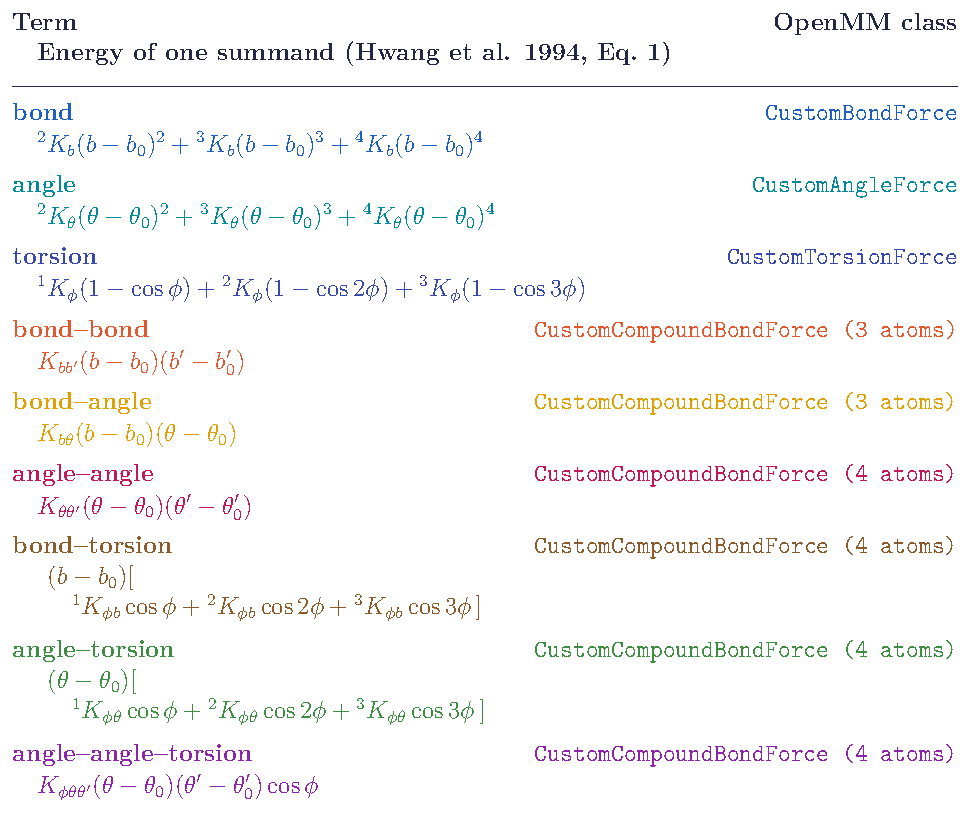
\includegraphics[width=\textwidth]{../figures/openmm-mapping-table.pdf}
\caption{Valence terms of CFF93 (Hwang et al.\ 1994, Eq.\ 1) and their OpenMM implementation. Each row is the energy of one bond, angle, torsion or pair; the total is the sum over all of them. Pasteable versions: \texttt{figures/openmm-mapping-table.svg/.png}.}
\label{fig:table}
\end{figure}

\paragraph{What each cross term captures.} The physical readings below are standard explanations of such couplings \emph{(not from a provided source)}; the paper supplies the forms and values.
\begin{description}
  \item[\tc{cBondBond}{bond--bond}] two bonds that share an atom: if one stretches, the neighbour tends to shorten or lengthen.
  \item[\tc{cBondAngle}{bond--angle}] a bond in an angle and the angle itself: the angle opens as the bond lengthens.
  \item[\tc{cAngleAngle}{angle--angle}] two angles on the same atom sharing a bond: opening one squeezes the other.
  \item[\tc{cBondTorsion}{bond--torsion}, \tc{cAngleTorsion}{angle--torsion}, \tc{cAngleAngleTorsion}{angle--angle--torsion}] the bonds and angles around a torsion depend on the rotation: eclipsed conformations are strained and stretch or open.
\end{description}

\paragraph{Which atoms enter each sum.} Eq.~1 writes double sums; Table~4 gives one constant per atom-type combination. In the code each distinct bond pair, angle pair or torsion is counted once, bond--torsion uses the central bond with its constants (Table 4 J) and both terminal bonds with theirs (Table 4 K), and angle--torsion uses both angles that belong to the torsion (Table 4 L). Angle--angle pairs are angles on the same central atom that share one bond (the paper's ``common bond'' column, Table 4 H). That the sums run exactly this way is my reading of Eq.~1 and Table~4, not an explicit statement in the part of the paper I read; the code tests only that OpenMM and an independent numpy implementation agree with each other.

\section{CFF93: scaling a quantum-mechanical surface}
The paper does not fit all force constants to experiment. It starts from constants derived from an ab initio energy surface and rescales them with five scale factors and two bond reference lengths (Eq.~2, Table~3): $S_b$ (0.88 for C--C, 0.83 for C--H), $S_\theta=0.81$, $S_\phi=0.84$, $S_c=0.87$ for all cross terms. The motivation is that Hartree--Fock force constants are roughly 10--15\% too large (p.~2517). The values used in the examples here are the final scaled constants of Table~4.

\section{OpenMM examples}
\texttt{class2\_openmm.py} builds each term as one OpenMM force in its own force group, so that the energy of each term can be read separately. Bonds, angles and torsions map onto \texttt{CustomBondForce}, \texttt{CustomAngleForce}, \texttt{CustomTorsionForce}. The cross terms involve several internal coordinates at once, so each is a \texttt{CustomCompoundBondForce} acting on three or four atoms, with the geometry written using the built-in \texttt{distance}, \texttt{angle} and \texttt{dihedral} functions. Parameters are the CFF93 alkane values of Table~4 converted to kJ/mol and nm. Nonbonded terms (Table 4 D, E) are not included. The checks (\texttt{test\_class2.py}) compare each term's OpenMM energy on a randomly displaced ethane and n-butane against a plain numpy implementation, and against hand numbers for a stretched C--C bond. These show the OpenMM code implements the equations as written; they do not validate CFF93 against experiment.

\section{Why this matters now}
Recent force-field work trains simple valence forms on large datasets. Blanco-Gonz\'alez et al.\ \cite{BlancoGonzalez2026} tried the Urey--Bradley angle term (a class II-like coupling of the outer atoms) and found it trained but did not beat the conventional harmonic form, and they name class II force fields as a future direction. OPLS5 \cite{Damm2024} extends a class I form with Drude polarisation rather than cross terms. Machine-learning potentials such as MACE-OFF \cite{Kovacs2025} avoid the choice of functional form altogether, at higher cost. Differentiable simulation \cite{Greener2025} is a way of training such functional forms against data. I have not found a PCFF or COMPASS form in the provided sources, so they are not covered here.

\bibliographystyle{unsrtnat}
\bibliography{refs}
\end{document}
